\renewcommand{\chapid}{intro}

\chapter{ Introduction \chaplabel{intro} }
%\addcontentsline{toc}{chapter}{Introduction}

%[Why do we need redshifts? cosmology problems and galaxy evolution, use as distance proxy via Hubble law]

Photometric redshift (\pz) estimation has been a staple of studies of galaxy evolution, large-scale structure, and cosmology since its conception decades ago \citep{Baum1962}.  
An extremely coarse spectrum in the form of photometry in a handful of broadband filters can be an effective substitute for the time- and photon-intensive process of obtaining a spectroscopic redshift (\sz), a procedure that may only be applied to relatively bright galaxies.  
Once the photometric colors are calibrated against either a library of spectral energy distribution (SED) templates or a data set of spectra for galaxies with known redshifts, a correspondence between photometric colors and redshifts may be constructed, forming a trustworthy basis for \pz\ estimation or testing.

Calculations of correlation functions of cosmic shears and galaxy positions that constrain the cosmological parameters require large numbers of high-confidence redshifts of surveyed galaxies.  
Many more \pz s may be obtained in the time it would take to observe a smaller number of \sz s, and \pz s may be measured for galaxies too dim for accurate \sz\ confirmation, permitting the compilation of large catalogs of galaxy redshifts spanning a broad range of redshifts and luminosities.  
\Pz s have thus enabled the era of precision cosmology, heralded by weak gravitational lensing tomography and baryon acoustic oscillation peak measurements.  

However, \pz s are susceptible to inaccuracy and imprecision via a number of effects, particularly their inherent noisiness due to the coarseness of photometric filters, catastrophic errors in which galaxies of one type at one redshift are mistaken for galaxies of another type at a different redshift, and systematics introduced by observational techniques, data reduction processes, and training or template set limitations.  
The projection of these physical and algorithmic effects into the space of true and estimated redshifts is discussed extensively in \Chap{pzdc1}, and their impact on cosmological parameter constraints is addressed in \Chap{chippr}, but some introductory material will motivate the following discussion.

\Fig{fig:pedagogical_scatter} illustrates the relationship between photometry and redshift generically by showing ``data'' in one dimension for visualization purposes, suggesting that a special nonlinear projection of the photometry could more-or-less yield a one-to-one relationship with true redshifts.
This plot looks very much like the traditional $z_{\mathrm{spec}}$ versus $z_{\mathrm{phot}}$ plots of traditional \pz\ point estimates and was indeed adapted from one such plot in \citet{jain_whole_2015}, because \pz\ point estimates effectively are a special nonlinear projection of the data.

\begin{figure*}
	\begin{center}
		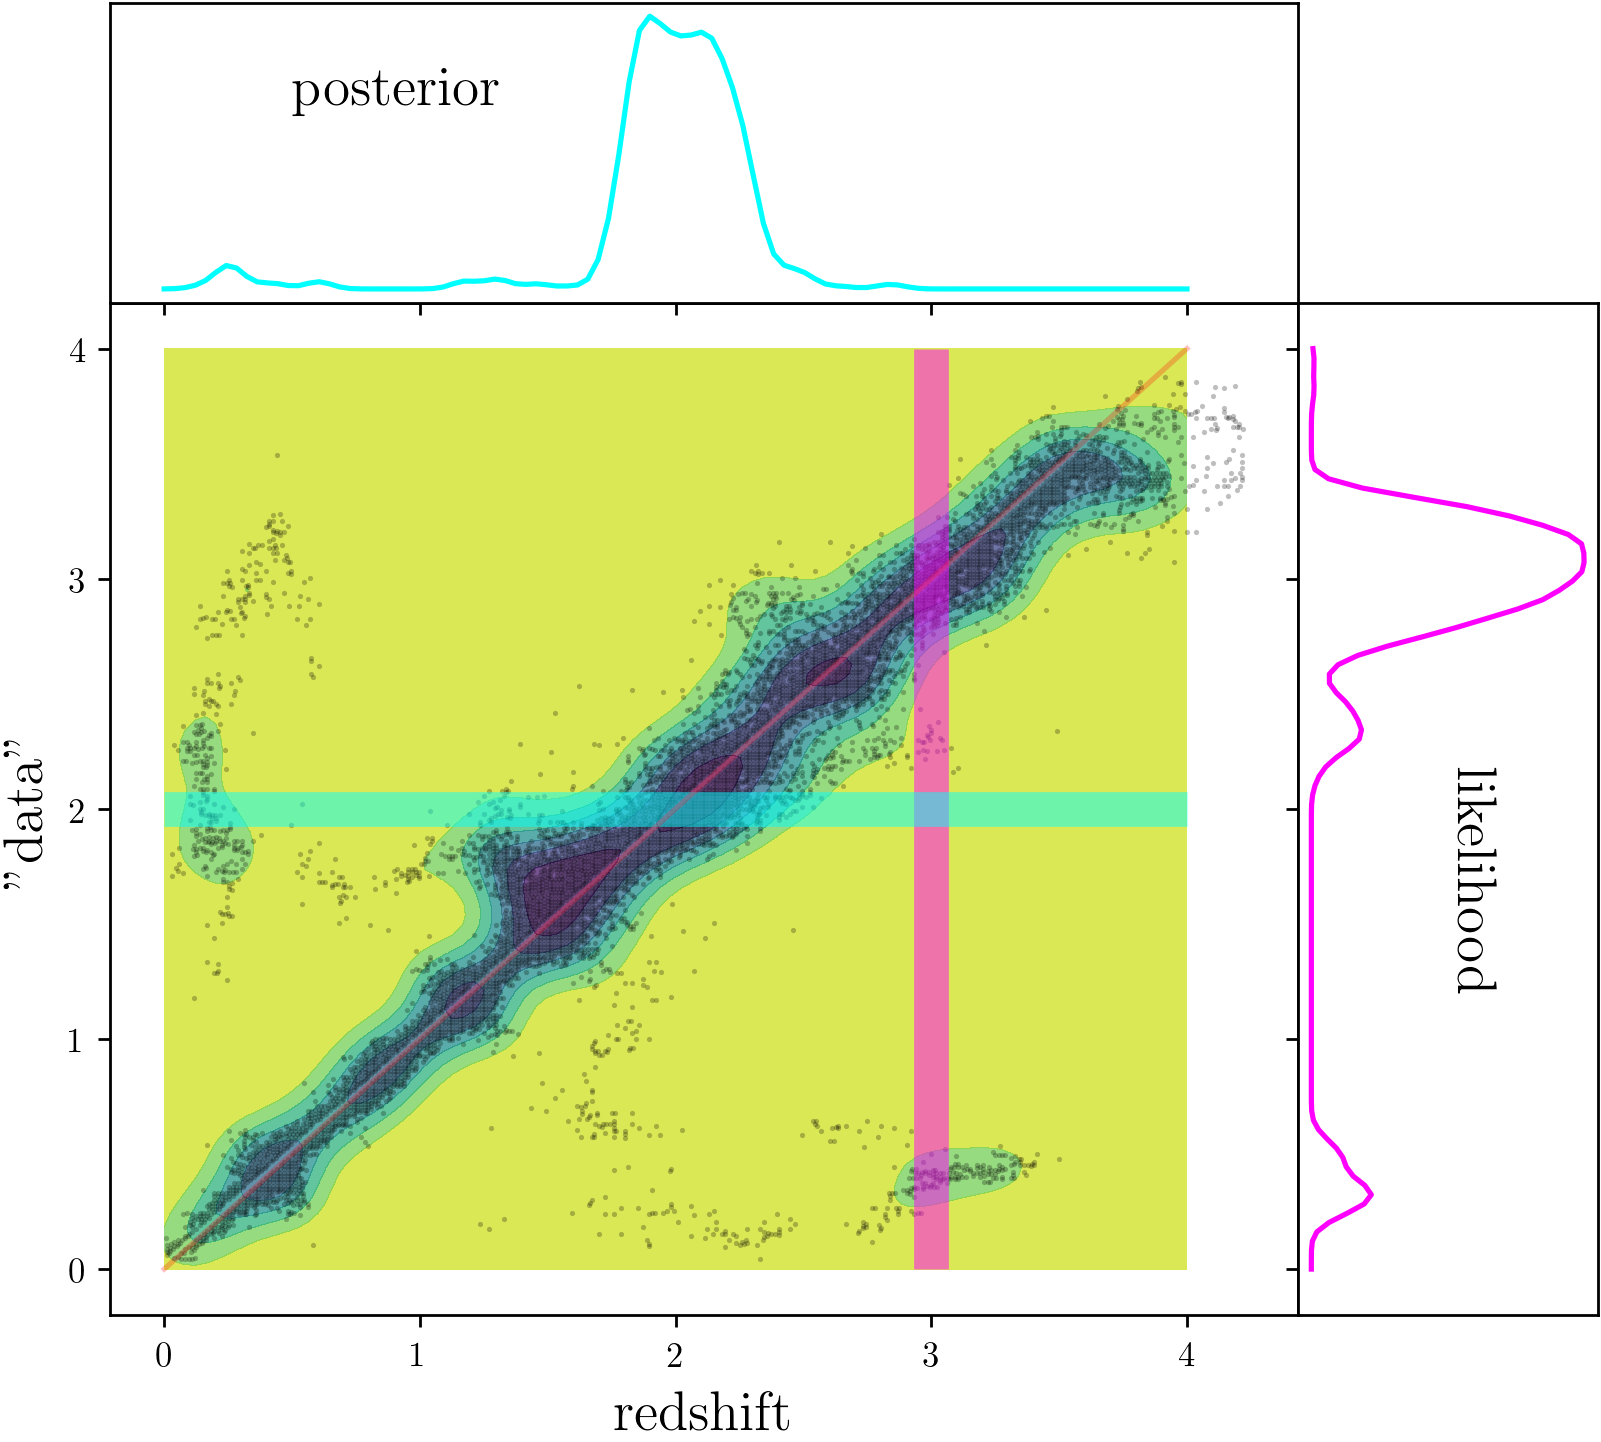
\includegraphics[width=0.74\textwidth]{figures/intro/jain05.png}
		\caption{
			A generic probability space (darker in areas of higher probability density) of redshift ($x$-axis) and data ($y$-axis), projected into a single dimension, with vertical cuts and marginals (cyan) indicating the construction of likelihoods and horizontal cuts and marginals (magenta) indicating the construction of posteriors.
			The data (black points) used to generate the contours were extracted from \citet{jain_whole_2015} using WebPlotDigitizer \citep{rohatgi_webplotdigitizer_2019}, with the ideal redshift estimation provided for reference (red diagonal).
%			\aim{Choose better colors?}
		}
		\figlabel{fig:pedagogical_scatter}
	\end{center}
\end{figure*}

There are several varieties of generally non-Gaussian deviation from a perfect correspondence between redshift and data in \Fig{fig:pedagogical_scatter}, represented by a $y = x$ diagonal line.
There is scatter about the diagonal due to the coarseness of the photometric filters, with larger scatter perpendicular to the diagonal due to the specific wavelengths where highly identifiable spectral features pass between the filters, as well as higher scatter at high redshifts due to larger photometric errors on fainter galaxies.
There are populations of outliers, far from the diagonal, comprised of galaxies for which the redshift estimate is catastrophically distinct from the true redshift, showing that outliers are not uniformly distributed nor restricted to long tails away from a Gaussian scatter.
And, though hardly perceptible in the plot, there is a systematic bias, wherein the average of the points would not lie on the diagonal but would be offset by a small amount, suggested by the trend of points to lie below the diagonal at high redshift.
Based on the goals of a photometric galaxy survey, limits can be placed on the tolerance to these effects.
For example, the Large Synoptic Survey Telescope (\lsst) states requirements for the main cosmological sample in the \lsst\ Science Requirements Document (SRD)\footnote{\url{https://docushare.lsstcorp.org/docushare/dsweb/Get/LPM-17}} \citep{Mandelbaum:2018}, reproduced in \Tab{tab:lsstsrd}.

\begin{table}
	\begin{center}
		\caption{\Pz\ requirements for \lsst\ cosmology \citep{Mandelbaum:2018}.}
		\tablabel{tab:lsstsrd}
	\begin{tabular}{ll}
		Number of galaxies & $\sim 10^{7}$\\
		Root-mean-square error & $\sigma_z < 0.02 (1 + z)$\\
		$3 \sigma$ catastrophic outlier rate & $< 10\%$\\
		bias & $< 0.003 (1 + z)$
	\end{tabular}
	\end{center}
\end{table}

In addition to these limitations in accuracy, there is also the matter of uncertainty quantification; \pz s are often reported with presumed-Gaussian error bars derived without the inclusion of all systematic errors, including the selection effects in the space of photometric colors or magnitudes that differ between the galaxies for which \pz s are desired and the galaxies with \sz s that are used to calibrate \pz\ estimators.
An example of this selection bias in the context of \project{zCOSMOS} \citep{lilly_zcosmos_2009} and \project{COSMOS} \citep{laigle_cosmos2015_2016} is shown in \Fig{fig:selection-bias}, which shows a distinct lack of support between the \project{COSMOS} and \project{zCOSMOS} galaxy populations in magnitudes and photometric redshift estimates.
This mismatch can bias one-point statistics of the affected galaxy populations \citep{moresco_spot_2013}, motivating the development of elaborate procedures to compensate for such bias in the context of two-point statistics of galaxy redshifts \citep{mandelbaum_precision_2008}.

\begin{figure*}
	\begin{center}
		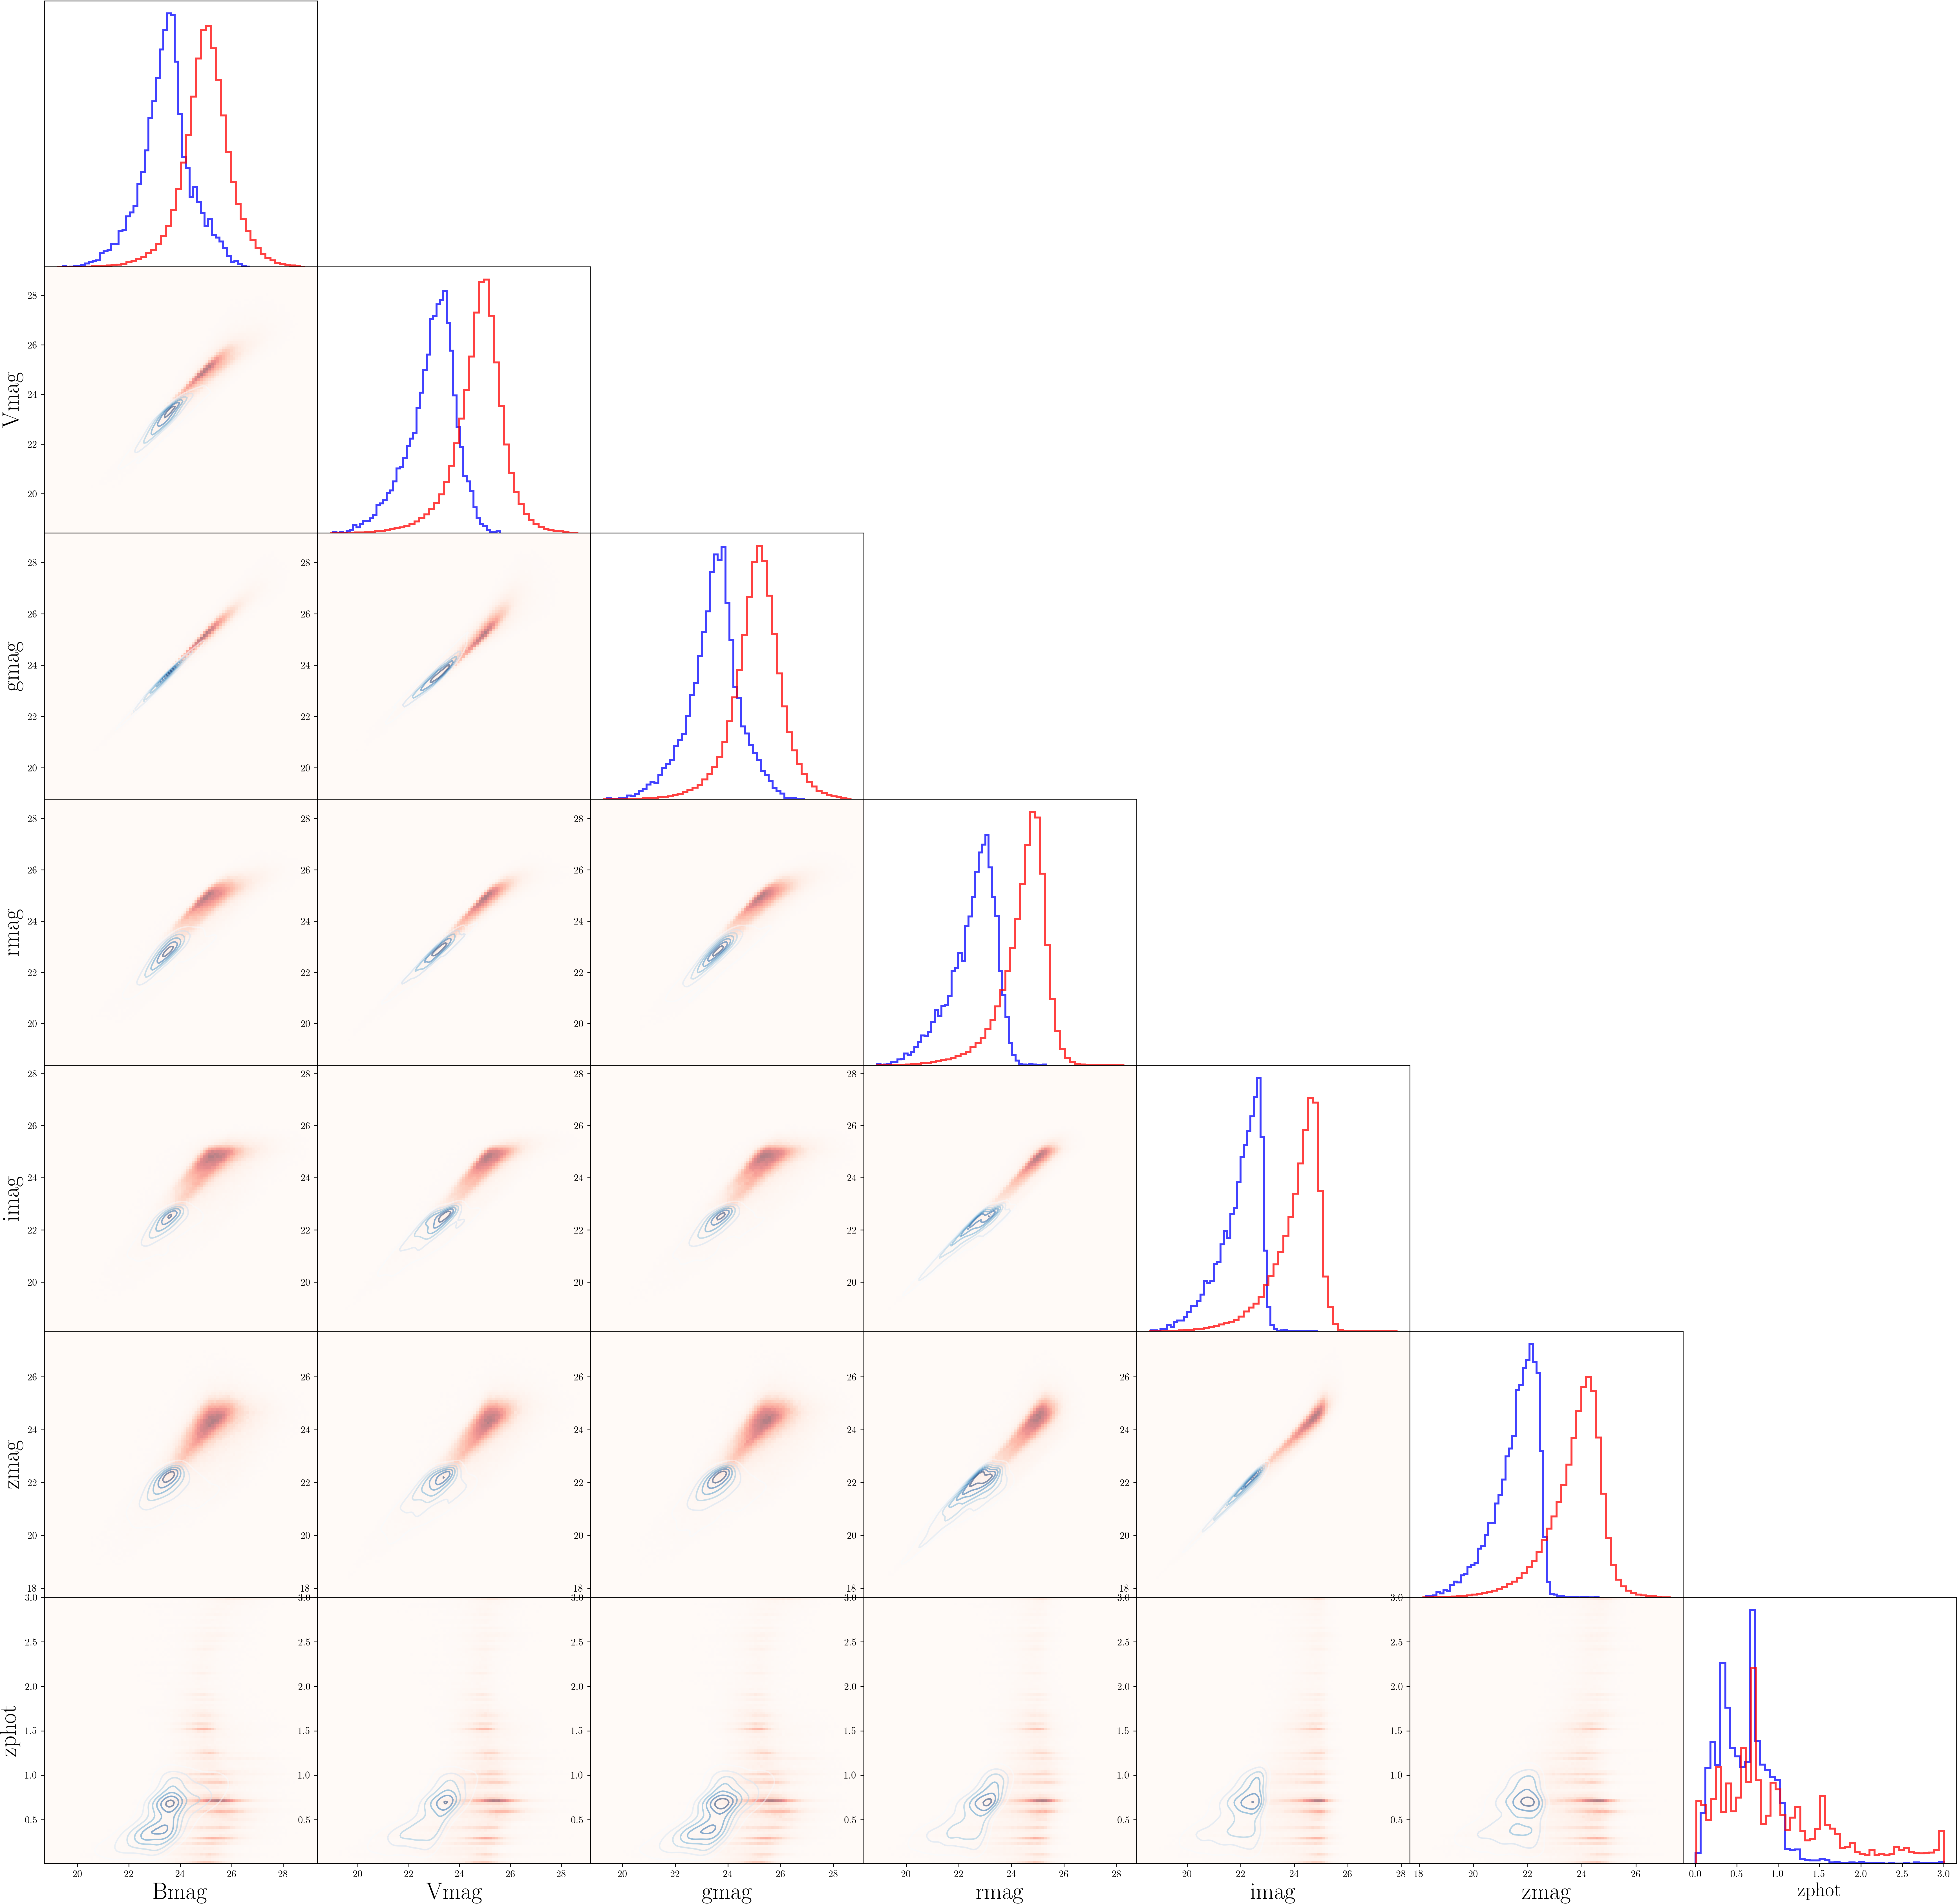
\includegraphics[width=0.99\textwidth]{figures/intro/big_corner_coarse.png}
		\caption{
			The distributions of magnitudes and the provided photometric redshift estimate for the galaxies with complete photometric data in \project{zCOSMOS} ($8,826$ galaxies; blue) and \project{COSMOS} ($395,019$ galaxies; red).
			It is evident that the sample for which spectra were unavailable is not well-supported by the sample for which spectra were obtained, which was used to calibrate the spectroscopically unconfirmed set.
%			\aim{I also have this plot for colors instead of magnitudes, which is a little less dramatic but still shows the lack of support.}
		}
		\figlabel{fig:selection-bias}
	\end{center}
\end{figure*}

Once propagated through the calculations of correlation functions of cosmic shear and galaxy positions, \pz\ errors are not insignificant contributors to the total uncertainties reported on cosmological parameters.
As progress has been made on the influence of other sources of systematic error, the uncertainties associated with \pz s have come to dominate the error budget of cosmological parameter estimates made by current surveys such as \des\ \citep{hoyle_dark_2017}, \project{HSC} \citep{tanaka_photometric_2018}, and \project{KiDS} \citep{hildebrandt_kids-450:_2017}.

Much effort has been dedicated to improving \pz s, though they are still most commonly obtained by a maximum likelihood estimator (MLE) based on libraries of galaxy SED templates, with conservative approaches to error estimation.
This approach tends to lead to catastrophic outliers like the horizontally oriented population of \Fig{fig:pedagogical_scatter}, due to the presence of galaxies whose SEDs are not represented by the template library.
Data-driven approaches tend to result in catastrophic outliers like the vertically oriented population of \Fig{fig:pedagogical_scatter}, due to training sets that are incomplete in redshift coverage.
Recent advances have focused on identifying and removing catastrophic outliers when using \pz s for 
inference \citep{Gorecki2014}.  
The approaches of using a training set versus a template library are related to one another by \citet{Budavari2009}.
Sophisticated Bayesian techniques and cutting-edge machine learning methods have been employed to improve precision \citep{Carliles2010} and accuracy \citep{sadeh_annz2:_2016}. 

An alternative to point estimation of \pz s is redshift probability distribution function (PDF) estimation that reports the probability $\pr{z}$ over all possible redshifts for every galaxy rather than an MLE (with or without presumed Gaussian error bars) \citep{Koo1999}.  
This option is favorable because it contains more potentially useful information about the uncertainty on each galaxy's redshift, incorporating notions of precision, accuracy, and systematic errors.
However, denoting \pzpdf s as ``$\pr{z}$'' is an abuse of notation, as it does not adequately convey what information is being used to constrain the redshift $z$; \pzpdf s are \textit{posterior} PDFs, conditioned on the photometric data and prior knowledge, as is covered in detail in \Chap{pedant}, as well as \Chap{chippr} and \Chap{pzdc1}.
In terms of \Fig{fig:pedagogical_scatter}, \pzpdf s are horizontal cuts, probabilities of redshift conditioned on a specific value of data, i.e. posteriors, which constrain redshifts, whereas vertical cuts through this space are probabilities of data conditioned on a specific redshift, i.e. likelihoods, from which data is actually drawn.

%\aim{what interesting problems/opportunities are the context for my work?  (drawing conclusions about the universe from vast quantities of uncertainty-dominated, limitations of photometry lead to methodological challenges, what was tried so far and why isn't it good enough)}

%\aim{what science can be done with that opportunity? (cosmology, and then some! the interesting problems are in testing LCDM, GR, inflation, also galaxy evolution)}

\Pzpdf s have been produced by completed surveys \citep{Hildebrandt2012, sheldon_photometric_2012} and will be produced by ongoing and upcoming surveys \citep{LSSTScienceCollaboration2009, CarrascoKind2014a, bonnett_redshift_2016, Masters2015}.  
\Pzpdf s are not without their own weaknesses, however, including the resources necessary to calculate and record them for large galaxy surveys \citep{CarrascoKind2014} and the divergent results of each method used to derive them \citep{Hildebrandt2010, Dahlen2013, Sanchez2013, bonnett_redshift_2016, tanaka_photometric_2018}.  
The most important of these issues, however, is that use of them in the literature is inconsistent at best and incorrect at worst.  
The most common application of \pzpdf s is their use in estimating \Nz, the distribution of redshifts of a sample of galaxies, a quantity essential to the calculation of the power spectra of weak gravitational lensing and large-scale structure that are used to constrain the parameters of cosmological models \citet{mandelbaum_precision_2008, sheldon_photometric_2012, bonnett_redshift_2016}.
%\aim{Provide equations/citations for the use of \Nz\ in cosmology.}

If the true redshifts $\{z_{i}^{\dagger}\}$ of galaxies $i$ were known, then the redshift PDFs would be delta functions $\{\delta(z, z_{i}^{\dagger})\}$ centered at the true redshift, and the redshift distribution could be effectively approximated by a histogram or other interpolation of the delta functions $\{\delta(z, z_{i}^{\dagger})\}$.
When \pzpdf s are available instead of true redshifts, the simplest approach reduces them to point estimates $\{\hat{z}_{i}\}$ of redshift by using $\delta(z, \hat{z}_{i})$ in place of $\delta(z, z_{i}^{\dagger})$.
Though it is most common for $\hat{z}_{i}$ to be the mode (maximum) of the \pzpdf, there are other, more principled point estimate reduction procedures \citep{tanaka_photometric_2018}.

To circumvent the reduction of uncertainty information due to point estimation, however, it has grown to be more common to calculate the mathematically inconsistent but conceptually simple \textit{stacked estimator} of the redshift density function \citep{Lima2008}, 
\begin{align}
\eqlabel{eqn:stack}
\hat{n}(z) &= \frac{1}{\ntot} \sum_{i = 0}^{\ntot} \pr{z}_{i}
\end{align}
for a sample of $\ntot$ galaxies $i$, or, equivalently, the redshift distribution function $\hat{N}(z) = \ntot \hat{n}(z)$.
Much of this thesis centers around the problems with this logically invalid yet pervasive quantity.

In \Chap{pedant}, I investigate how this blatantly incorrect estimator of the redshift distribution could become and remain widely accepted by the astronomical community.
I approach the problem from a mathematically rigorous perspective to identify the assumptions necessary for the stacked estimator to recover the true \Nz\ and note that because those assumptions will not hold for future surveys, including \lsst, we must use an alternative estimator that self-consistently propagates redshift uncertainty.

I go on to present one such alternative to stacking, the Cosmological Hierarchical Inference with Probabilistic Photometric Redshifts (\Chippr) model, in \Chap{chippr}.
\Chippr\ is a Bayesian hierarchical model that encapsulates the causal relationships between the redshift distribution of a galaxy sample, the redshifts of the individual galaxies, and each galaxy's photometric data.
I also present the publicly available \chippr\footnote{\url{https://github.com/aimalz/chippr}} code that implements the \Chippr\ model and includes a comprehensive suite of tools for testing arbitrarily realistic mock \pzpdf\ catalogs.
Using \chippr\ and the \cosmolike\footnote{\url{https://github.com/CosmoLike}} forecasting suite, I show that stacking causes a substantially higher information loss on \nz, corresponding to broader 1-$\sigma$ error ellipses on the cosmological parameters, whereas \chippr is unbiased if the method used to obtain the \pzpdf s is well-characterized.

In order for the approach proposed in \Chap{chippr} to be applied, there must be a \pzpdf\ catalog, yet many techniques to obtain \pzpdf s have been proposed and tested in the literature without clear indications that one is superior to all others.  
An extension of the Bayesian photometric redshift (BPZ) method of \citet{Benitez2000} that produces posterior probability distributions (as opposed to a selection of local maxima) from an SED template library has been employed \citep{Hildebrandt2012, Kelly2014, Lopez-Sanjuan2015}.  
\Pzpdf s have also been obtained by a variety of trustworthy data-driven approaches in the literature: $k$-nearest neighbor algorithms with \citep{Ball2008} and without \citep{sheldon_photometric_2012} inclusion of photometric measurement errors, neural networks \citep{bonnett_using_2015}, self-organizing maps \citep{CarrascoKind2014a}, and prediction tree and random forest classification techniques \citep{Carliles2010, CarrascoKind2013}.  

Of course, this brief review does not cover all ways to obtain \pzpdf s; many more may be found in the literature, along with comparisons thereof \citep{Hildebrandt2010, Dahlen2013, Sanchez2013, bonnett_redshift_2016, tanaka_photometric_2018}.
Some current work aims to vet \pzpdf\ generation methods not only from a perspective of comparing as many methods as possible but also by recognizing the importance of the comparison metric used to judge the performance of each algorithm \citep{Wittman2016, polsterer_dealing_2016}.
\Chap{pzdc1} details the comparative investigation of Schmidt, Malz, and Soo, et al. 
%(\aim{Figure out how to cite this as in review with a link to the public draft?}) 
but goes beyond the scope of previous attempts to identify the best \pzpdf\ technique by critiquing the evaluation criteria themselves from a mathematically principled perspective.
By proposing a new \pzpdf\ estimation technique, \trainz, I demonstrate the pitfalls of all performance metrics previously used in evaluating \pzpdf\ techniques in the literature and highlight the conditional density estimation loss as a promising option when true \pzpdf s are not available for comparison.

In the absence of an obvious best choice for the method used to derive \pzpdf s, \lsst\ has planned to provide to the community several \pzpdf s per galaxy obtained by a variety of methods rather than choosing one, effectively hedging bets on which may ultimately prevail.
This goal of storing multiple \pzpdf s, however, must be accomplished without exceeding the available data storage capacity of the survey nor compromising the integrity of subsequent science applications due to loss of information in the compression and reconstruction schemes.
\Chap{qp} approaches the problem of choosing how best to store \pzpdf s such that the results of multiple \pzpdf\ techniques may be available to the scientific community, focusing in particular on the number of stored parameters under different possible parameterizations of stored \pzpdf s.

To recap, \Chap{pedant} isolates the conditions under which stacking is actually valid, showing that the necessary assumptions were to a limited extent true for early galaxy surveys but are violated by modern missions and will not be upheld whatsoever in the future, motivating the migration to new methods.
\Chap{chippr} presents one such method, a mathematically rigorous methodology for inferring \Nz\ from a catalog of \pzpdf s, including the effect of propagating an incorrectly inferred \Nz\ to constraints on the cosmological parameters.
\Chap{pzdc1} comprehensively compares twelve approaches to probabilistic photometric redshift estimation, presenting novel discoveries of the impact of the assumptions implicit to the method by which the redshift probabilities are derived and the limitations of established performance metrics of such probabilistic data products in assessing the quality of the procedures for deriving them.
\Chap{qp} concerns how redshift probabilities are to actually be used, answering the question of how probabilistic data products should be stored and delivered to users in order to enable valid science, as well as how to go about answering that question for a generic science application.

\chapname~\chapalt{pedant} is original material developed initially as lecture notes and ultimately intended for submission to PRD.
The contents of \chapname~\chapalt{chippr} have been presented at numerous conferences, and a video representation of it was awarded finalist status in the 2018 Dance Your Ph.D. Competition, but it remains a public draft accompanied by the \chippr\footnote{\url{https://github.com/aimalz/chippr}} code not yet submitted for publication.
\chapname~\chapalt{pzdc1} is a second-author paper currently under \desc\ internal review and publicly available online\footnote{\url{https://github.com/LSSTDESC/PZDC1paper}}, with intended submission to MNRAS.
\chapname~\chapalt{qp} is a first-author paper that has been refereed and published in AJ \citep{malz_approximating_2018}, and the \qp\footnote{\url{https://github.com/aimalz/qp}} code produced for the study is published and citeable \citep{malz_qp_2017}.

Here, I describe my specific contributions to each \chapname\ and acknowledge the contributions of my co-authors:
\begin{enumerate}

{\item For \chap{pedant}, I conducted the entire investigation, though Phil Marshall (SLAC) originally posed the question, albeit with different phrasing.}

{\item For \chap{chippr}, I led the development, implementation, and validation of \Chippr, initially under the guidance of David Hogg (NYU) and later continued to work on all three aspects of the project under the supervision of Phil Marshall (SLAC).}

{\item For \chap{pzdc1}, I led the choice, evaluation, and interpretation of the comparison metrics, I devised and implemented the \trainz\ technique of \pzpdf\ estimation, and I wrote a substantial fraction of the text.
	Sam Schmidt (UC Davis) led the overall study, coordinating contributions from most of the \Pz\ Working Group of the \desc; a detailed enumeration of the role of each of over twenty co-authors is provided in \Chap{pzdc1}.}

{\item For \chap{qp}, with encouragement from Phil Marshall (SLAC), I devised the idea for the project, designed the experiment, implemented and validated the \qp\ code, conducted the investigation, and wrote the paper.
	The mock data was produced by Sam Schmidt (UC Davis), Melissa Graham (UW), Joe DeRose (Stanford), and Risa Wechsler (Stanford).}

\end{enumerate}
